\section{Experiments}
\label{sec:experiments}

\subsection{Experimental Setup and Evaluation Protocol}
The main experiments adopt Cityscapes~\cite{cordts2016cityscapes} $\rightarrow$ DensePASS~\cite{ma2021densepass}: Cityscapes serves as the labeled source domain, DensePASS as the unlabeled target domain, with its validation set used to evaluate adaptation from perspective street scenes to panoramic street scenes. The model is OmniSAM~\cite{zhong2025omnisam} / sam2\_s~\cite{ravi2025sam2}, using a 13-class protocol; all main results are from single random seed full protocol, without cross-dataset or multi-seed conclusions. Source domain labels are used for supervised segmentation loss, target domain training phase does not use human annotations; DensePASS validation labels are only used for model evaluation. Baseline and Ours adopt the same data list, preprocessing, and validation pipeline, differing only in whether MTC and SMR are enabled during the training phase.

This paper uses mIoU to measure class-level segmentation quality, and reports mAcc, PixAcc, FWIoU, and mDice; BFScore supplements measurement of boundary consistency. mIoU reflects average region overlap across classes, while BFScore is more sensitive to ERP seams, elongated structures, and local boundary errors; together they characterize the quality cost of token reduction. Efficiency metrics include training time and iteration time. Memory Attention Time and Memory Tokens are only used in fixed pseudo-label ablation settings and cannot be mixed with end-to-end training time.

\subsection{Implementation Details}
MTC and SMR are placed before memory attention, separately changing memory spatial density and retrieval subset, without modifying source domain supervision, target domain pseudo-label loss, or segmentation output. Main results compare OmniSAM with Ours (MTC+SMR). The latter simultaneously uses auxiliary confidence masks during training, but the paper's main name highlights MTC and SMR which directly change memory computation; pseudo-label generation phase maintains the original pipeline to avoid mixing training efficiency gains with pseudo-label changes. PQR is independent as a pseudo-label reliability auxiliary ablation.

\subsection{Main Results}
\begin{table}[t]
  \centering
  \small
  \setlength{\tabcolsep}{4pt}
  \renewcommand{\arraystretch}{1.08}
  \caption{Segmentation performance and training efficiency comparison under Cityscapes $\rightarrow$ DensePASS full protocol. All results use \texttt{sam2\_s}, 13-class protocol, and single random seed setting; BFScore comes from \texttt{[ValSummary]} of the same validation pipeline.}
  \label{tab:main_results}
  \begin{tabular}{lccccc}
    \toprule
    Method & mIoU$\uparrow$ & BFScore$\uparrow$ & Train Time$\downarrow$ & Iter Time$\downarrow$ & Reduction \\
    \midrule
    OmniSAM & \textbf{60.26} & \textbf{39.97} & 43m53s & 5.27s & -- \\
    Ours (MTC+SMR) & 60.16 & 39.86 & \textbf{34m03s} & \textbf{4.09s} & \textbf{22.4\%} \\
    \bottomrule
  \end{tabular}
\end{table}


Table~\ref{tab:main_results} shows that Ours (MTC+SMR) has mIoU and BFScore 0.10 and 0.11 lower than OmniSAM, respectively. The slight accuracy and boundary cost indicates that token reduction is not lossless, but major segmentation quality remains stable, supporting the existence of compressible redundancy in historical memory. Changes in region and boundary metrics are close in magnitude, with no large-scale prediction failure; since a single random seed is used, these differences should still be viewed as observations under this protocol.

\subsection{Efficiency Analysis}
Table~\ref{tab:main_results} also provides end-to-end training efficiency: Ours (MTC+SMR) reduces both training time and iteration time by approximately 22.4\%. This gain comes from reducing the token scale entering memory attention. End-to-end time includes computation beyond memory, so its reduction is smaller than what pure attention modules might achieve, but better reflects actual cost of complete UDA training. This result only indicates training phase efficiency; this paper does not verify inference acceleration or memory reduction.

\subsection{Qualitative Results}
Figure~\ref{fig:qualitative_full_protocol} compares OmniSAM baseline with MTC+SMR. Both maintain similar major scene structures, with differences remaining in local boundaries and small objects, consistent with slight BFScore degradation; these examples serve only as qualitative observations.

\begin{figure}[t]
    \centering
    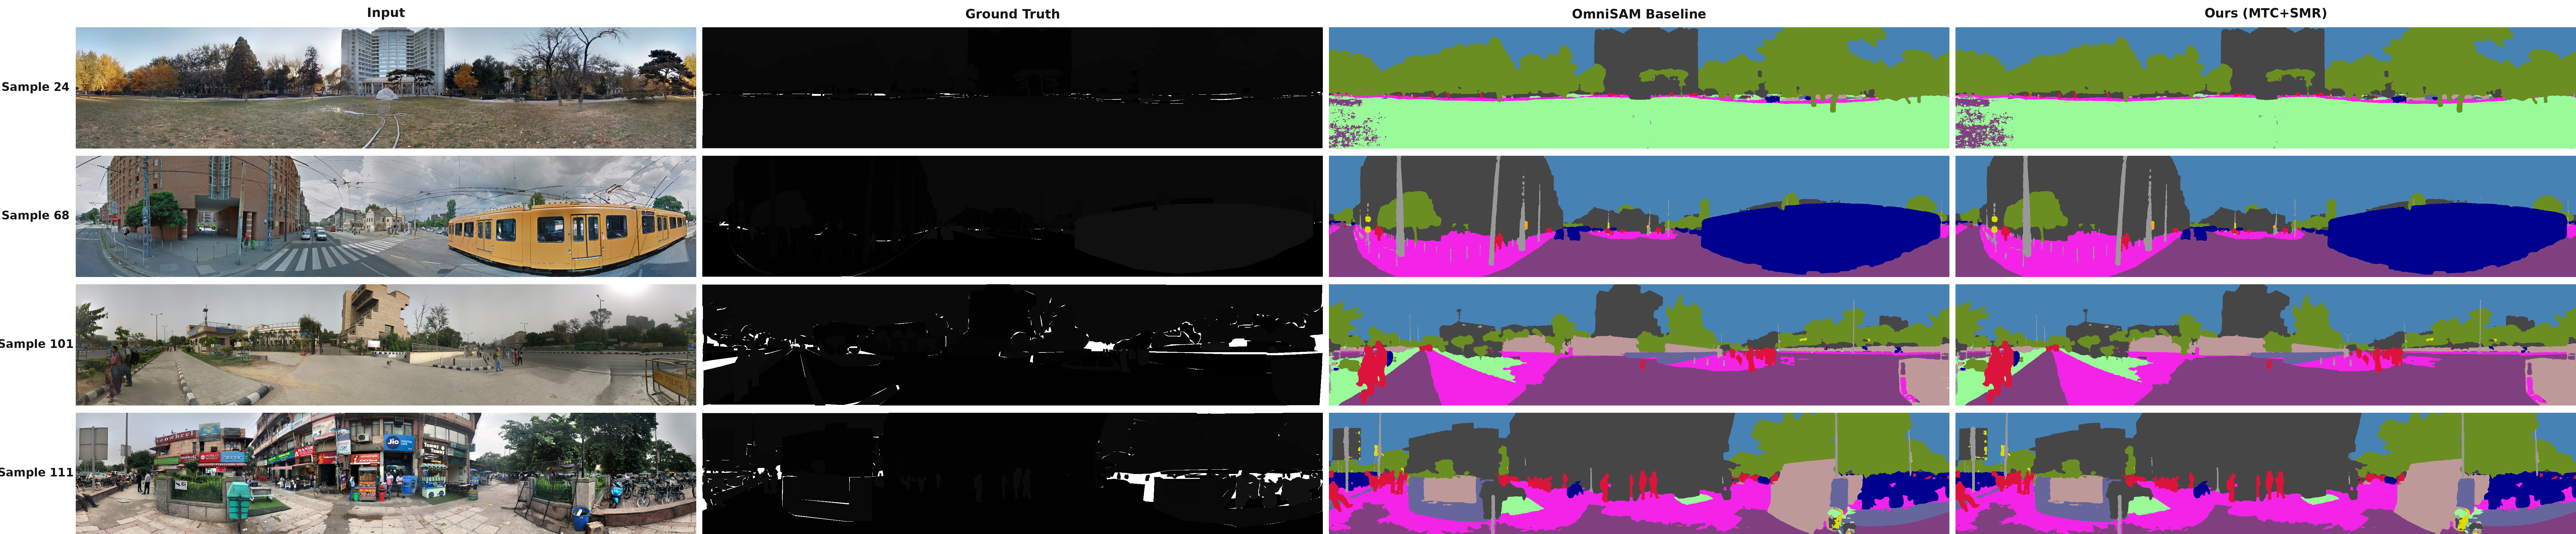
\includegraphics[width=\linewidth]{figures/fig_qualitative_full_protocol.png}
    \caption{Qualitative segmentation results under Cityscapes $\rightarrow$ DensePASS full protocol. Each row shows target domain input, ground truth, OmniSAM baseline prediction, and our MTC+SMR configuration prediction. Baseline and Ours use the same sam2\_s, 13-class protocol, data preprocessing, and ERP inference pipeline.}
    \label{fig:qualitative_full_protocol}
\end{figure}
